\documentclass[a4paper]{jpconf}
\usepackage{graphicx}
% \usepackage{color}
% \usepackage{array}
% \usepackage{enumerate}

% To create a graphic:
% 1) save your image as a 1024x1024 png/gif/bmp
% 2) convert to pdf (install ImageMagick, then 'convert FileIn.png FileOut.pdf')
% 3) to resize the image, if needed, 'convert FileIn.png -resize 66% FileOut.pdf' etc
% N.B. if the input and output files have the same base name, LaTeX will prefer to take the png
% over the pdf, which is probably not what you want. Make sure the files have different names!
%\begin{figure}[htp]
%\centering
%\includegraphics{file-basename}
%\caption{figure caption blah blah}\label{fig:figure-ref}
%\end{figure}

\begin{document}
\title{Comprehensive Monitoring for Heterogeneous Geographically Distributed Storage}

\author{Ratnikova~N$^1$, Karavakis~E$^2$, Lammel~S$^1$, and Wildish~T$^3$}

\address{$^1$ Fermi National Accelerator Laboratory, US}
\address{$^2$ CERN, CH}
\address{$^3$ Princeton University, US}

\ead{natalia.ratnikova@cern.ch, tony.wildish@cern.ch}

\begin{abstract}


Storage capacity at CMS Tier-1 and Tier-2 sites reached over 100 Petabytes in 2014, and will be substantially increased during Run 2 data taking. The allocation of storage for the individual users analysis data, which is not accounted as a centrally managed storage space, will be increased to up to 40\%. For comprehensive tracking and monitoring of the storage utilization across all participating sites, CMS developed a Space Monitoring system, which provides a central view of the geographically dispersed heterogeneous storage systems. The first prototype has been deployed at the pilot sites in summer 2014, and has been substantially reworked since then. In this presentation we discuss the functionality and our experience of system deployment and operation on the full CMS scale.

\end{abstract}
\section{Introduction}

CMS experiment computing \cite{cmscomptdr} infrastructure spans over more than a hundred 
of geographically distributed sites that provide both computational and data storage 
resources. Storage capacity at the sites varies from hundreds terabytes to several petabytes. 
During the first LHC run, CMS data saturated hundred petabytes of storage. 
Data taking rate and total data volume will be substantially increased during the Run 2.

% include CMS site map

Storage accounting and space monitoring becomes increasingly important for data 
management tasks, such as efficient space utilization, fair share between users and 
groups, and resource planning. 

Data stored at the sites are coming from a variety of sources and include i) centrally managed 
data sets such as real detector data and simulated data samples at various stages of reprocessing, 
software release validation samples; ii) files created by individual 
users or members of physics analysis groups stored at the associated institute sites; 
iii) temporary unmerged files generated as part of the data processing workflows; 
iiii) load test and backfill data used for availability and scalability testing \cite{scalability}.

CMS space monitoring system, SpaceMon \cite{spacemon}, provides monitoring for storage space 
occupied by various directories in the CMS data directory tree. 

Information is retrieved directly from the local site storage systems in the form of 
storage dumps produced by various methods or tools depending on the storage technology and
local sites infrastructure, following a commonly agreed format \cite{LHCstorageaccouting}.

The CMS data management system \cite{cmsdatamanagement} keeps track the centrally managed 
file replicas in the central data transfer management database. The SpaceMon information 
collected at the sites allows to account additional storage space used by the users 
and groups, and various other volatile data areas, not tracked in the central catalogs.

The information is aggregated locally at the sites, then uploaded into a central database at CERN.

In the next section we discuss site information providers process and tools.
Section 3 and 4 describe spacemon client software and the components of the central infrastructure.
In conclusion we present current status and our experience of SpaceMon deployment at CMS sites.

\section {Site information providers}


To provide storage usage information for the space monitoring system, CMS sites 
are asked to produce storage dumps in one of the predefined formats, currently 
text or XML. These formats were chosen based on WLCG recommendations described 
in \cite{storagedumps}.  Each line of the dump file contains  XML  tags or fields 
separated by a vertical bar with the following values: physical file name as 
addressed on the site storage file system, files size in bytes, optional: 
file creation date and checksum. The time stamp of the dump creation is provided 
in a separate XML tag, or encoded in the dump file name.
Once created, the storage dump is processed by CMS provided SpaceMon client tool, 
which aggregates file sizes and creates a space usage record including directory 
sizes up to a certain level of depth. 

CMS sites use various storage technologies for maintaining CMS data, including:
Castor, dCache,DPM, EOS, Hadoop, LStore, Lustre, StoRM. There is no unique 
solution for retrieving the local storage information for all sites. 

On the posix-like file systems, such as EOS, Lustre, Hadoop systems mounted 
with FUSE, or NFS-mounted dCache storage, the {\it find} command can do the work.
However traversing the whole storage namespace by this method may cause extra 
load on the system, or take long time to execute. For some storage systems, 
e.g. dCache, direct database query on namespace database is more efficient
while causing less load. The impact on the production storage system can be
completely avoided when storage dumps are produced on the hot standby server, 
onto which the namespace database is dynamically replicated for a backup. 
Sites that provide storage to multiple experiments, can optimize by dumping 
only a sub-branch of the namespace under CMS-owned directory. 
Another possible optimization is to aggregate directory sizes on the database 
level instead of producing the whole storage dump. SpaceMon client provides 
an API to read in the aggregated record. 

The choice of the information provider tools remains with the site admins. 
In many cases the successful recipe can be reused with minimal configuration
adjustments. CMS site admins exchange tools and solutions for creating storage 
dumps via an open source repository on github. Fig. \ref{fig:github_stats} shows
statistics of commits to the repository for the last year. 

\begin{figure}[h]
\center
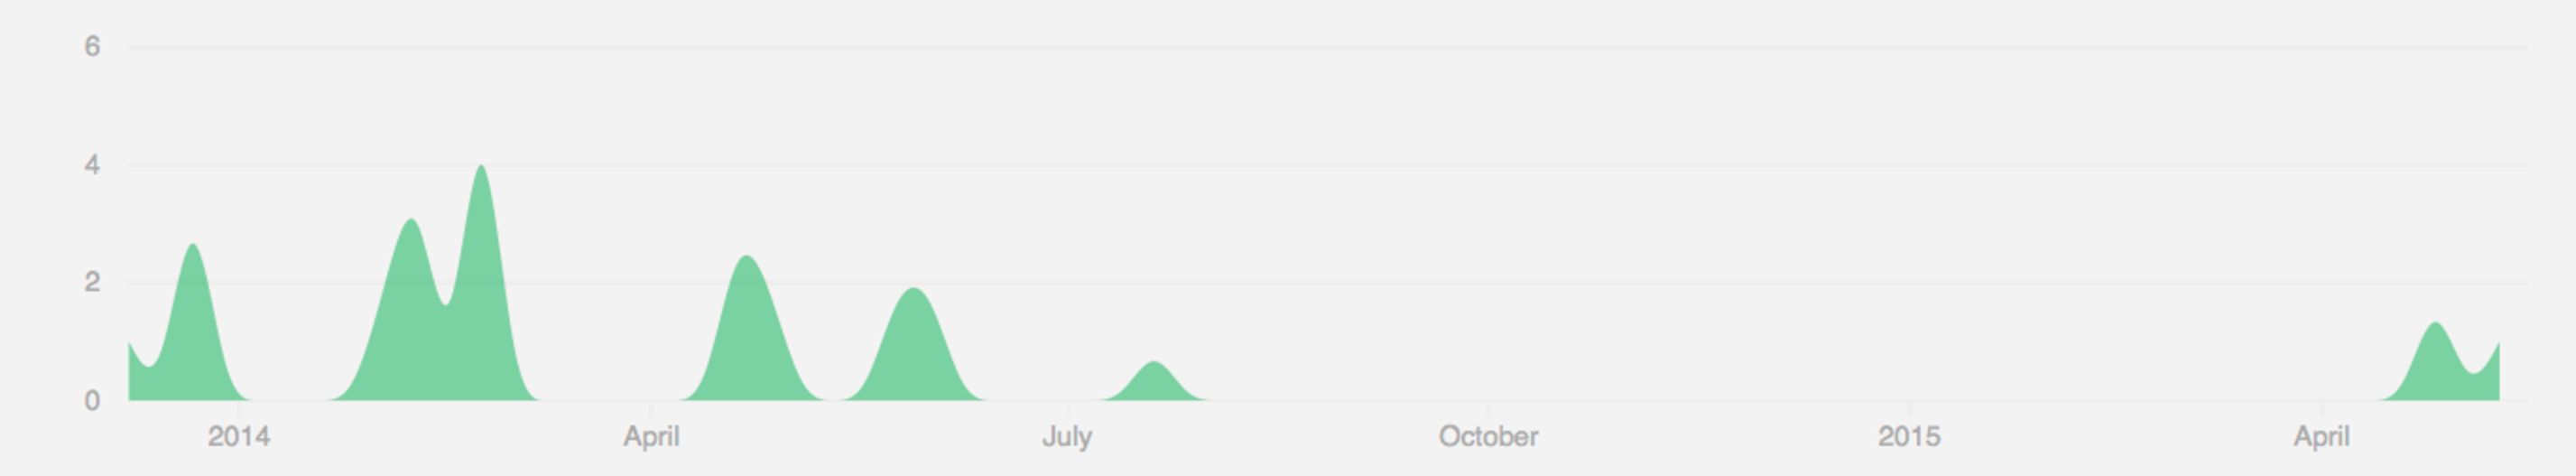
\includegraphics[width=1.0\linewidth]
{pictures/sites_contributions.pdf}
\caption{Commits contributed by CMS site admins to SiteInfoProvider tools repository}
\label{fig:github_stats}
\end{figure}


\section {Site client software}

\section {Central infrastructure}


\subsection {DMWMMON Database as Information store}


\subsection {Data Service as interface to Information store}

\subsection {SiteDb as authentication authority}



\subsection {DashBoard as es end-user visualization tool}

The goal of the visualization is to present the space monitoring information 
in a convenient form, enabling users to check space usage across the sites, 
explore historical views or drill down into a particular directory in the 
CMS storage namespace. While this functionality is required for the central data 
operations and CMS overall storage resource management and utilization, it is
also useful for the site administrators and individual storage users. We opted 
for WLCG Experiment Dashboard \cite{ExpDashboard} framework for the
implementation of space monitoring visualization. CMS dashboard, basd on this 
framework, already provides visualization for monitoring job processing, data 
transfers and site/service usability.

Recently started work with WLCG dashboard developers resulted in the architecture 
proposal shown in Figure 2.
\begin{figure}[h]
\center
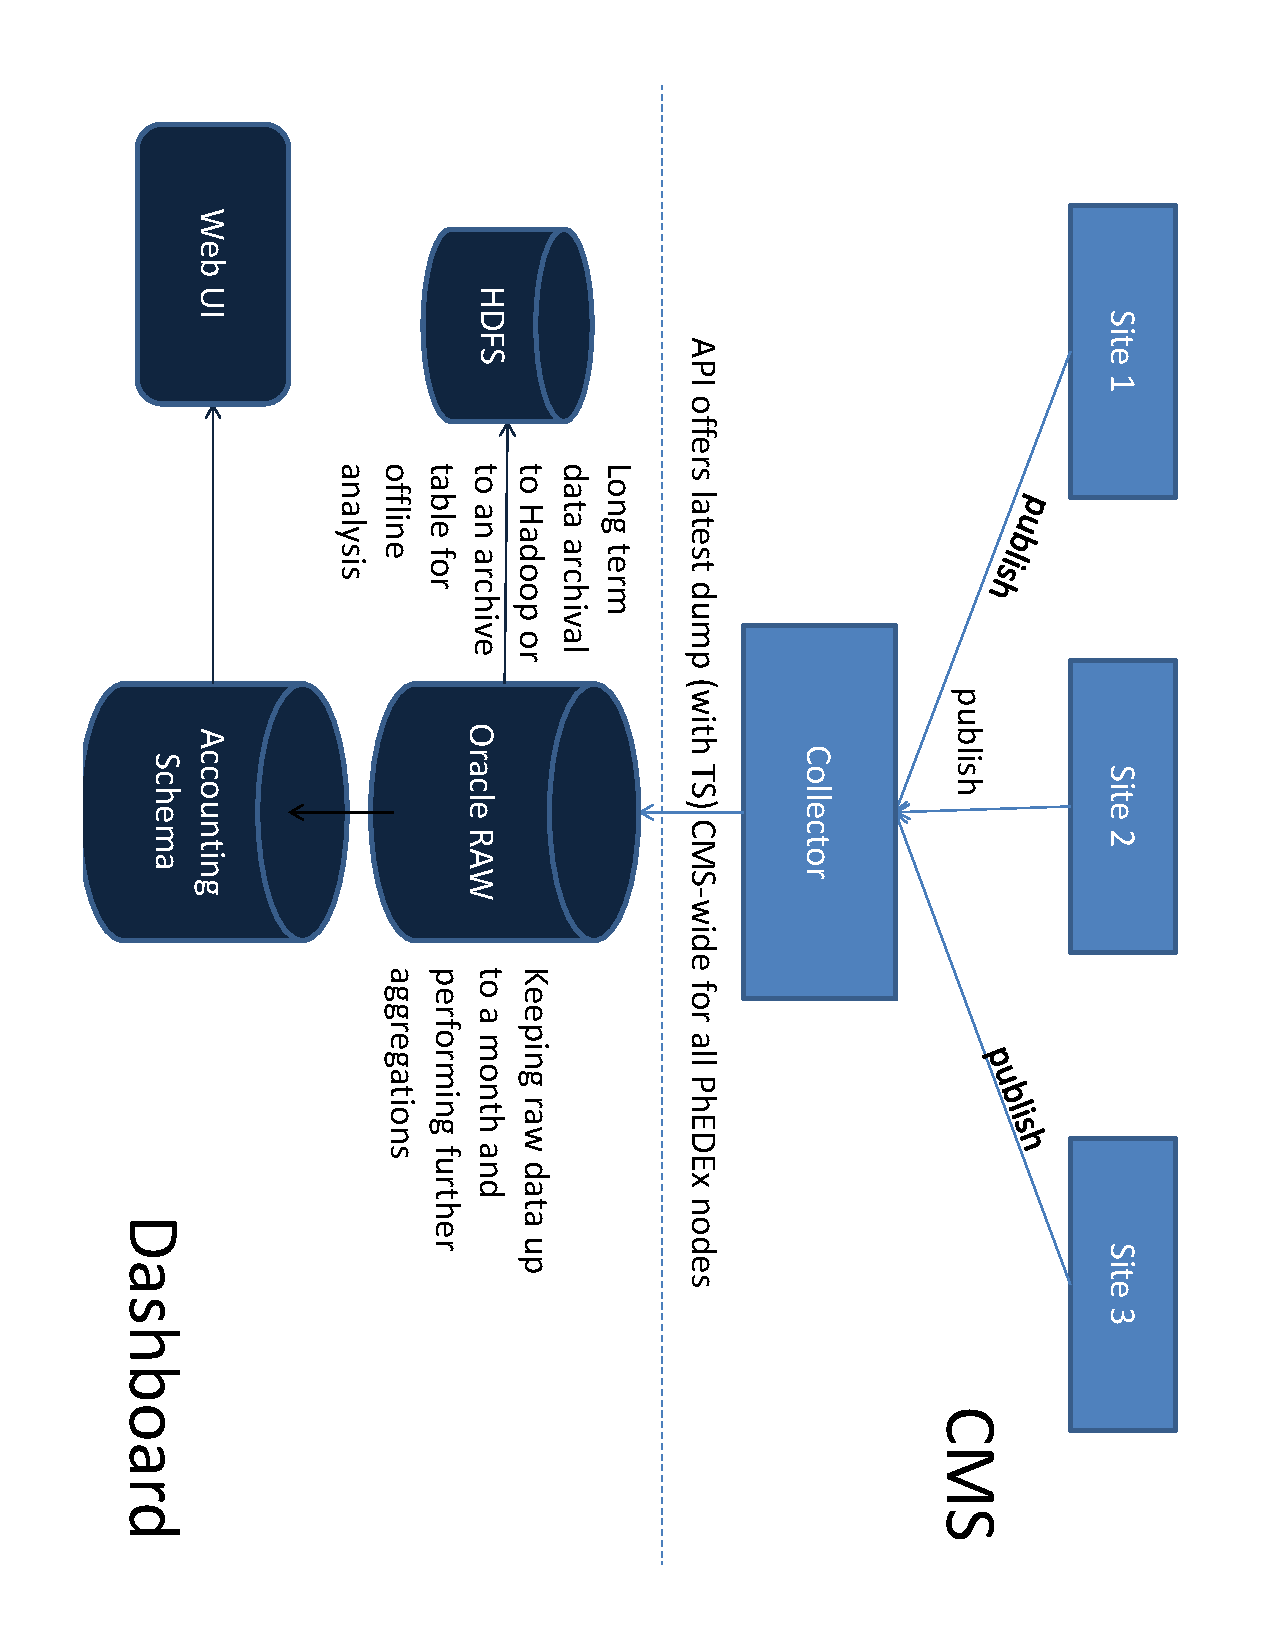
\includegraphics[width=0.8\linewidth, angle =90]
 {pictures/SpaceMonVisProposal-p1.pdf}    
\caption{Proposed architecture for storage accounting and visualization 
in CMS Dashboard based on CMS Space Monitoring information}
\label{fig:vis_proposal}
\end{figure}

Similar design was developed and deployed for ATLAS storage accounting \cite{DDMAccounting}
based on storage summaries from the central data management catalogs. The challenge in CMS 
case is to represent uniformly the monitoring data asynchronously pushed by the sites.

\section{Deployment}

The deployment of the first prototype started in late spring of 2014.
A few pilot sites with close association to project members were
chosen and contacted. The goal of this campaign was to collect and
upload to the central data service the storage information from a few
sites. This allowed to independently verify the provided client
software tools and that the documentation is complete and well
structured. It also provided some first data that could be used to
design and test the visualization tools. Administrators from several
sites contributed with feedback and improvements in this first test.
The pilot deployment led to enhancements in the central data service
and to updates of the documentation.

In February of 2015 CMS computing management decided to proceed with
the role out of the space monitoring. CMS site support setup a metric
in the CMS dashboard that monitors the space information uploaded by
sites. When this was ready, sites were contacted in small batches and
ask to setup regular uploading of storage information to the central
data service. About ten site administrators were contacted via email
each week. This allowed to sort out any remaining hidden issues, fine
tune instructions, and provide prompt response to questions and in
case of problems. The last sites were contacted beginning of May. The
issues encountered during this first stage of this deployment can be
categorized into three groups: 1) Questions from sites about why they
need to provide storage usage information and at what level of detail;
2) Authentication problems uploading the information to the central
data service; 3) The long time it takes to take a dump for some
storage systems. Sites were informed about how CMS plans to use the
storage information. Site were reminded about the three main reasons
for the space monitoring project: i) consistency checks between site
storage and central PhEDEx catalogue, ii) monitoring the inventory of
areas that are not managed by PhEDEx, and iii) to apply user and group
quotas fairly at the experiment lavel, i.e.\ across sites. For level
of detail on the storage information guidance was provided and the
documentation clarified. The by far largest issues were related to
the authentication to upload the information. Instructions and also a
script to troubleshoot the authentication problems has been provided.
In the process we found the perl-based upload client to not function
correctly with the one of the perl-SSL libraries and a problem with
the curl command in the current Scientific Linux distributions. On
some large storage systems a dump can take several days to complete
and this needs to be accounted for. As of middle May 2015, about half
of the sites are uploading space information regularly. Several sites
are in the process of setting it up. There are no outstanding
technical issues preventing sites from providing space information.
The plan is to follow the first stage with a ticketing campaign for
any remaining sites. We anticipate the roll out to be completed in
June.

With plans to enhance the schema of the central data service, sites
have been ask to keep the storage dumps they currently take. Given
the upload issues, we are also looking into at other secure upload
solutions.

\section {Summary}

% \input{section-....tex}
% \input{section-....tex}

\par
\section*{References}

\begin{thebibliography}{1}

%Intro: 
\bibitem{cmscomptdr} Bonacorsi D {\it et al.} 2007 The CMS computing model 
{\it Nucl. Phys.} B {\it (Proc. Suppl.)} {\bf 172} 53-56

\bibitem{scalability}
 Belforte S {\it et al.} 2010 Bringing the CMS distributed computing system into scalable operations 
{\it J. Phys.: Conf. Ser.} {\bf 219} 062015

\bibitem{spacemon}
N Ratnikova {\it et al.} 2014 CMS Space Monitoring {\it J. Phys.: Conf. Ser.} {\bf 513} 042036 

\bibitem{storagedumps}
Huang C-H {\it et al.} 2012 Data Storage Accounting and Verification at LHC experiments 
{\it J. Phys.: Conf. Ser.} {\bf 396} 032090

\bibitem{cmsdatamanagement}
M Giffels {\it et al.} 2014 The CMS Data Management System {\it J. Phys.: Conf. Ser.} {\bf 513} 042052


\bibitem{PhEDEx}
  Egeland R, Wildish T and Metson S 2008 Data transfer infrastructure for CMS data taking,  
{\it XII Advanced Computing and Analysis Techniques in Physics Research (Erice, Italy: Proceedings of Science)}


% central infrastructure section: 
% Tony's references for SiteDB and Data Service 

\bibitem{SiteDB} 
Metson S {\it et al.} 2010 SiteDB: marshalling people and resources available to CMS
{\it J. Phys.: Conf. Ser.} {\bf 219} 072044

% For DMWMMON DB and data-service, you can refer to them as based on the PhEDEx data-service:

\bibitem{DataService} 
 R Egeland {\it et al.} 2010  PhEDEx Data Service 
{\it J. Phys.: Conf. Ser.} {\bf 219} 062010

% References for visualization from Eddie: 
\bibitem{ExpDashboard} 
  Andreeva J {\it et al.} 2012 Experiment Dashboard - a generic, scalable solution for 
monitoring of the LHC computing activities, distributed sites and services 
{\it J. Phys. Conf. Ser.} {\bf 396} 032093

\bibitem{DDMAccounting} 

Karavakis E {\it et al.}  2014 Common Accounting System for Monitoring the ATLAS 
Distributed Computing Resources
{\it J. Phys.: Conf. Ser.} {\bf 513} 062024

%references from CHEP2012 paper:
\bibitem{wlcg} Knobloch J {\it et al.} 2005 "LHC Computing Grid Technical Design Report" CERN-LHCC-2005-024
\bibitem{ATLASDDM} Garonne V, Molfetas A, Lassnig M, Barisits M, Stewart G A, Beermann T 2012 "The ATLAS Distributed Data Management project: Past and Future", these proceedings
\bibitem{SRM} Shoshani A,  Sim A and  Gu J 2002 ``Storage Resource Managers: Middleware Components for Grid Storage'',  Nineteenth IEEE Symposium on Mass Storage Systems'
\bibitem{cms} The CMS Collaboration 2008 "The CMS experiment at the CERN LHC" JINST {\bf 3} S08004
\bibitem{DBS3} Giffels M and Guo Y Data Bookkeeping Service 3 - A new event data catalog for CMS, submitted to CHEP 2012
\bibitem{phedex} Egeland R, Wildish T and Metson S 2008 "Data transfer infrastructure for CMS data taking" {\it XII Advanced Computing and Analysis Techniques in Physics Research} (Erice, Italy: Proceedings of Science)
\bibitem{filelight} Ball G 2011 PhD thesis, chapter 8 ``Computing Monitoring Pages",
 https://workspace.imperial.ac.uk/highenergyphysics/Public/theses/Ball.pdf
\bibitem{d3} The D3 javascript library http://mbostock.github.com/d3/
\bibitem{LHCbDiracFramework} Stagni F {\it et al.} 2012: "LHCbDIRAC: distributed computing in LHCb",  these proceedings 
\bibitem{SLS} Lopienski S 2008 ``Service level status - a new real-time status display for IT services'' {\it J. Phys.: Conf. Ser.}  {\bf 119} 052025
%\bibitem{SRMspecs}  Sim A and Shoshani A 2009 The Storage Resource Manager Interface Specification Version 2.2,  https://sdm.lbl.gov/srm-wg/doc/SRM.v2.2.html


%\bibitem{LFCandDPM}  "Official Documentation for LFC and DPM"  https://twiki.cern.ch/twiki/bin/view/LCG/DataManagementDocumentation  
\bibitem{LFC} Baud J-Ph et al 2005 Performance analysis of a file catalog for the LHC computing grid HPDC
14 91-99
\bibitem{LHCbDiracBookkeeping} Charpentier P  {\it et al.} 2012 "The LHCb Data Management System",  these proceedings 
\bibitem{Serfon:2010zz} 
  Serfon C 2010
  "Data management tools and operational procedures in ATLAS: Example of the German cloud,"
  J.\ Phys.\ Conf.\ Ser.\  {\bf 219}, 042053 (2010).
  %%CITATION = 00462,219,042053;%%
\bibitem{Magini:2011zz} 
  N.~Magini, N.~Ratnikova, P.~Rossman, A.~Sanchez-Hernandez and T.~Wildish,
  "Distributed data transfers in CMS,"
  J.\ Phys.\ Conf.\ Ser.\  {\bf 331}, 042036 (2011).
  %%CITATION = 00462,331,042036;%%
\bibitem{ElisaTwiki} Lanciotti E 2011 "Storage elements dumps and consistency checks versus file catalogues"
https://twiki.cern.ch/twiki/bin/view/LCG/ConsistencyChecksSEsDumps
\bibitem{Sciaba:chep2012}Bauerdick L and Sciaba A 2012 "Towards a global monitoring system for CMS computing", these proceedings
\bibitem{syncat} Millar P {\it et al.} 2010 ``Dealing with orphans: Catalogue synchronisation with SynCat'' J. Phys.: Conf. Ser. 219 062060
\bibitem{namespace} Sanchez-Hernandez A, Egeland R, Huang C-H, Ratnikova N, Magini N and Wildish T, 2012 "From toolkit to framework - the past and future evolution of PhEDEx", these proceedings
\bibitem{castor} Castor, http://castor.web.cern.ch/castor/
\bibitem{dcache} dCache,  http://www.dcache.org/
\bibitem{dpm} DPM (Disk Pool Manager) https://twiki.cern.ch/twiki/bin/view/LCG/DataManagementDocumentation\#DPM
\bibitem{eos} Peters A-J  2011 ``The EOS disk storage system at CERN'',  ACAT conference proceedings
\bibitem{bestman} BeStMan ( Berkeley Storage Manager) https://sdm.lbl.gov/bestman/
\bibitem{lustre} Lustre http://www.lustre.org/ 
\bibitem{lstore} L-Store (Logistical Storage)  http://www.accre.vanderbilt.edu/mission/services/lstore.php
%\bibitem{storm} StoRM (Storage Resource Manager),  http://storm.forge.cnaf.infn.it/
\bibitem{storm-gpfs}  Cavalli A  {\it et al} 2010  ``StoRM-GPFS-TSM: A new approach to hierarchical storage management for the LHC experiments''  {\it J. Phys.: Conf. Ser.} {\bf 219} 072030
\bibitem{xrootd} XRootD,  http://xrootd.slac.stanford.edu/
\bibitem{protovis} The Protovis javascript library http://mbostock.github.com/protovis/
\bibitem{highcharts} The Highcharts javascript library http://www.highcharts.com/

\bibitem{matplotlib} Matplotlib python 2D plotting library http://matplotlib.sourceforge.net/


\end{thebibliography}

% References from the poster: 

%1.http://iopscience.iop.org/1742-6596/396/3/032090/pdf/jpconf12_396_032090.pdf 
%2.https://github.com/dmwm/DMWMMON/tree/master/SiteInfoProviders
%3. https://twiki.cern.ch/twiki/bin/view/CMSPublic/SpaceMonSiteAdmin 
%4.http://dashb-ssb.cern.ch/dashboard/request.py/siteview#currentView=test
%5. http://dashb-atlas-ddm-acc.cern.ch/dashboard/request.py/ddmaccounting 
%6.http://rucio-hadoop.cern.ch/rucio/accounting/



\end{document}


Pro:Comprehensive Monitoring for Heterogeneous Geographically Distributed Storage
